\chapterimage{Figures/aux_optics.png} % Chapter heading image
%PMC bench in the 10m AEI prototype copyright AEI
\chapter{Auxiliary Optics}
%\section{Auxiliary Optics}
\label{sec:Aux-optics}

We use the term \emph{auxiliary optics} here for any optical subsystem not otherwise covered by a specific category (e.g. core optics or light sources). We further sub-categorize into these subsystems:
The {\bf Input Optics} subsystem includes all optics between the light source and the input of the core interferometer, typically defined by the power recycling mirror. The {\bf Output Optics} subsystem includes all optics between the core interferometer output (typically defined by the signal recycling mirror) and the photo-detectors which detect the gravitational wave signal, with the exception of specific optical components used for the generation of squeezed light. The {\bf Active Wavefront Control} subsystem includes means for sensing and actively controlling the spatial properties of interferometer beams, with the typical goal of minimizing mode matching losses and contrast defects. The {\bf Stray Light Control} subsystem encompasses all design features which are intended to reduce the impact of stray light on the detector operations. Finally, the subcategory {\bf Other Auxiliary Optics} catches optical subsystems that fall neither into the other larger categories or the aforementioned auxiliary optics subcategories.

\section{State of the art}
The {\bf Input optics} subsystem is responsible for delivering the laser light from the pre-stabilized laser (PSL) system to the core interferometer in the correct spatial mode, with the necessary phase modulation sidebands, as well as with the required frequency, intensity and alignment stability conditions. This subsystem therefore typically includes an electro-optic modulator (EOM) for producing the phase modulation, one or more suspended input mode cleaner (IMC) cavities, a power control system, and a input Faraday isolator (IFI) to protect the PSL from light reflected from the main interferometer. Detailed descriptions of the IO subsystems of aLIGO and AdVirgo can be found in Refs.~\cite{aLIGO_IO} and~\cite{IOchapter} respectively. 

\noindent
In 2G detectors, the {\bf Output optics} subsystem is responsible for filtering out higher-order spatial modes and unwanted control sidebands from the interferometer output light, and delivering the beam to the photodetectors where the GW signal measurement is made. The recent and planned squeezed light upgrades expand the role of this subsystem to include delivery of the squeezed beam to the main interferometer. This subsystem typically includes an output Faraday isolator, an output mode cleaner cavity (OMC), and high quantum efficiency photodiodes.

\noindent {\bf Active Wavefront Control} (AWC) is used in GW detectors to compensate for thermal effects caused by the absorption of light in the interferometer core optics. As the circulating light power goals increased from 1st to 2nd generation detectors, so too did the requirements for compensation of these thermal effects. The 2G detectors have all implemented a range of active wavefront control methods including ring heaters, CO$_2$ laser heating, thermal radiation projection, and thermally deformable mirrors~\cite{aLIGO_AWC, AdVirgo_IO}. This subsystem is often conflated with the thermal compensation system (TCS), although TCS constitutes only a part of the AWC system. 

\noindent {\bf Stray Light Control}
mitigates the effects of light scattered out of the main beam and then scattered back into it as that can cause noise that can limit the sensitivity of the detector.
To address this problem, many precautions are taken in GW detectors to minimize the amount of light scattered out of the beam (by using high-quality smooth optical surfaces everywhere), and also to minimize the available paths for re-entry of scattered light into the main beam (by using baffles wherever possible). 

\noindent 
Examples for the category {\bf "Other Auxiliary Optics"} include auxiliary length sensing (ALS) systems for pre-stabilizing the arm cavities, and optical levers for local sensing of the alignment of optics.

\section{Requirements, challenges and current/planned R\&D}
\subsection{Input optics}
 % Future 3G GW detectors will require different input optics than the current second-generation detectors. 
 The ways in which the 3G detector input optics will differ from the current ones depends heavily on some of the design decisions for 3G detectors, many of which have not yet been made. Most critical for the input optics will be the choice of laser wavelength; the EOM and IFI rely on unusual electro- and magneto-optic materials that may have significantly different characteristics at longer wavelengths. Choosing suitable materials is not expected to pose a great challenge if the wavelength is changed to 1550\,nm, but 2+$\mu$m will probably require considerable effort. The high power transmitted through these optics makes low absorption critical (due to the resulting thermal lensing and depolarization effects), thus further narrowing the choice of suitable material. At 2$\mu$m Faraday isolators already exist~\cite{EOTFI}, but a high power vacuum compatible one must be developed as it is not commercially available. Iron garnets should be considered as potential candidates for the magneto-optic material for 2+$\mu$m light, also having the advantage that the Faraday rotation effect is an order of magnitude larger than that of TGG in the near infrared range, allowing a reduction in magnet size and the overall footprint and weight of the device.
The IMC design is not expected to fundamentally change beyond the 2nd generation.  However, AdVirgo and aLIGO have both seen that noise contributions have been limited by beam jitter~\cite{aLIGOjitter,adVirgojitter}. Increasing the IMC finesse or adding a second IMC in series with the first could be a way to further suppress the beam jitter. Another possibility is to reduce the beam jitter at the source, either passively or with high bandwidth control loops.  

In addition to upgrades and modifications of existing IO components, several new components are also being researched. High bandwidth electro-optic beam deflectors could be used as actuators for beam jitter suppression loops and for providing alignment sidebands for an alternative method of alignment sensing in both the IMC and in the core interferometer~\cite{RFJASC}. The use of higher-order modes for coating thermal noise reduction is still under consideration for 3G interferometers~\cite{LGmodes}. If this technology is pursued further, the higher-order mode conversion/preparation path is likely to be incorporated into the IO remit. 

The use of complex modulation~\cite{complexmod} and parallel modulation~\cite{kagraMZI} are also under investigation for reducing sidebands-of-sidebands effects that may limit interferometer sensing and control performance.

\subsection{Output optics}
With all 3G concepts assuming significant enhancement from the use of squeezed light, the critical feature for the 3G output optics will be ultra-low optical losses~\cite{squeeze_lossbudget}. OFIs with reduced optical losses are being developed~\cite{EGOLLFI,UFLLFI}, for use in the advanced GW detectors. Figure~\ref{fig:AdVLLFI} shows the low-loss OFI which has recently been installed in Advanced Virgo. OMCs must also be designed for high throughput, and photodetectors must have high quantum efficiency (QE). High-QE photodetectors at longer wavelengths has been identified as a crucial R\&D task; one which may be especially onerous for 2+$\mu$m light. Frequency dependent squeezing will also require the inclusion of a filter cavity (FC) in the path between the squeezed light source and the OFI. 300\,m long FCs are planned for the near-term upgrades to aLIGO and AdV, following on from R\&D performed at MIT~\cite{MITFC} and in Japan\cite{TAMA_FDS2016}. Alternative readout schemes such as balanced homodyne detection (BHD - another project planned for inclusion in A+) will require a redesign of the output optics chain~\cite{BHD}. There is also a need to develop robust length and angular control schemes for detuned filter cavities.
% and finesse control to control pole frequency.

\begin{figure}[htb]
\centering
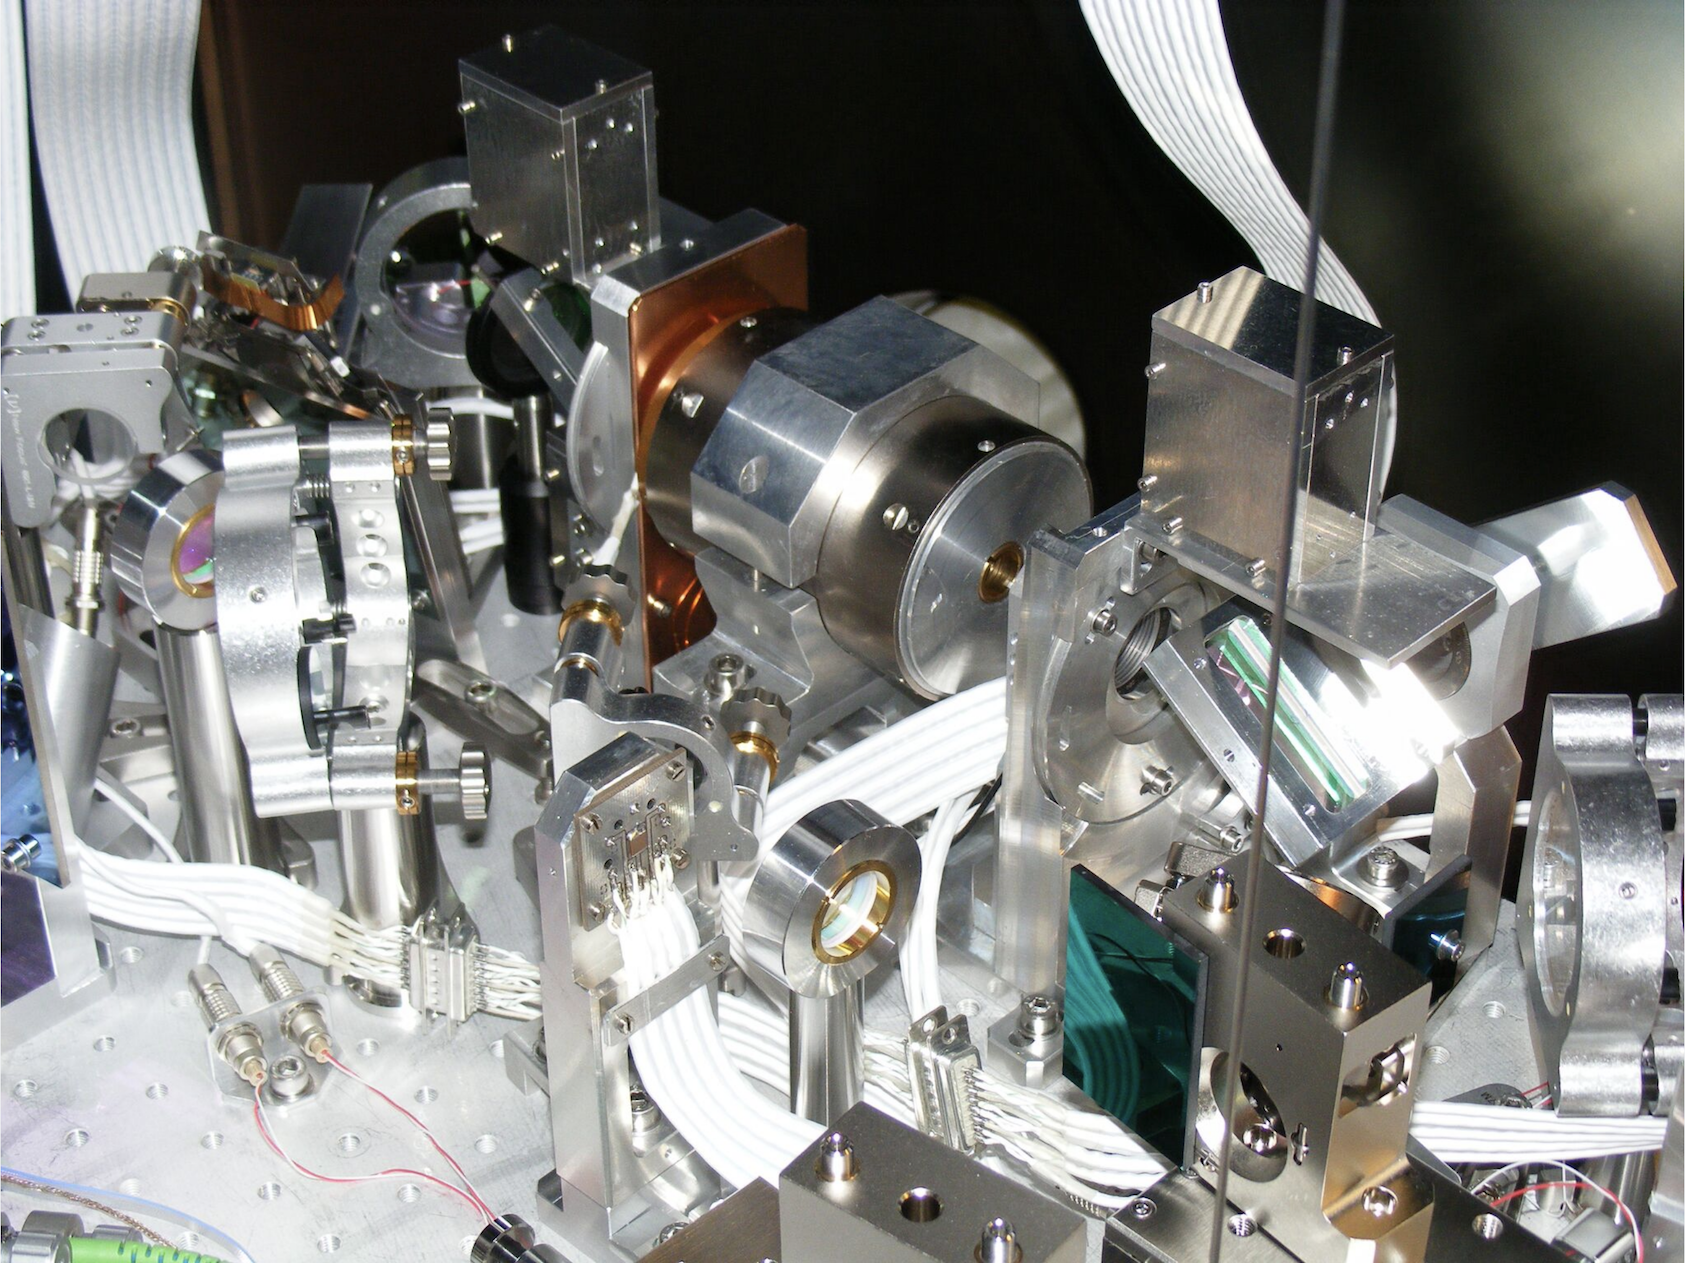
\includegraphics[width=0.6\textwidth]{Figures/LLFI.png}
\caption{The low-loss OFI upgrade to Advanced Virgo, recently installed ahead of the third observing run of the advanced detector era.\label{fig:AdVLLFI}}
\end{figure}

\subsection{Active wavefront control}
In 1st and 2nd generation detectors, active wavefront control (AWC) has often been implemented in something of an \emph{ad hoc} way. In no cases has a feedback loop been used to maintain mode matching in a detector during normal operations. This is partly due to the low bandwidth of the typical actuators, but also due to the limitations in the AWC sensors available. As a result, AWC is typically employed in a set-and-forget manner, which requires frequent manual retuning as the circulating power in the interferometer changes. 3G detectors will likely require higher performance from the AWC subsystem for several reasons: higher circulating powers, larger thermal gradients under cryogenic operation, larger beams with flatter wavefronts, and stricter requirements on optical losses. An LSC white paper on AWC has been written to track the LSC R\&D in this direction~\cite{aLIGO_AWC}, and similar work is planned for AdV+. AWC R\&D for 3G detectors is expected to focus on new sensors (RF bullseye wavefront sensors~\cite{bullseye}, improved Hartmann wavefront sensors~\cite{HWS}, phase cameras~\cite{phasecam}), as well as actuators (converting existing actuators for new optic materials, and developing new actuators). 

\subsection{Stray light control}
Although it is often difficult to diagnose directly, stray light was expected to be  limiting the sensitivity of both aLIGO and AdVirgo during O2. As such, improvements must clearly be made in order to reach 3G sensitivities with any methods other than extending the baseline length. Continued R\&D into mirror polishing and coating techniques to give improved surface roughness will go some way to reducing stray light contributions, as will the development of better baffling materials with lower reflectivities. One concern is that if the laser wavelength is changed to 2+$\mu$m, finding good absorbers for baffle materials may become more difficult. 

\subsection{Other auxiliary optics}
AdVirgo, aLIGO and Kagra all either use (or provision for) an auxiliary length sensing system in order to make the interferometer locking process deterministic. Since the optical layout of 3G detectors is not expected to reduce in complexity, it seems natural that similar systems will be required in the future. Optical levers are  omnipresent in 2G detectors, and provide important information about angular motion of the optics. Increased sensitivity in these local sensors may be beneficial for 3G detectors with increased baselines and sensitivity goals, and accordingly R\&D is ongoing towards that end. Suspension point interferometry (SPI)~\cite{SPI} may be a useful technique for reducing low frequency control noise in 3G detectors, and will require an additional auxiliary optical subsystem. SPI is currently being used at the AEI 10\,m prototype interferometer.   

\section{Current R\&D activities, pathways, required facilities, collaborations\\ and mechanisms}
A survey of research groups who are known to be working on, or have previously worked on auxiliary optics topics has been conducted~\cite{AuxActivitiesTable}.

Much of the auxiliary optics subsystems R\&D, such as materials investigations for EOMs and FIs, can be performed in small laboratories. 
Some of the larger subsystems such as filter cavities, on the other hand, require larger integrated facilities for testing. In many cases, the development of 3G auxiliary optics technologies is also beneficially incorporated into the modernisation of second-generation detectors. By virtue of being \emph{auxiliary}, modular, incremental upgrades in many of these technologies are possible. Modular upgrades are not feasible in the case of a change in the main laser wavelength, however. Such a change for 3G detectors will necessitate a broader range of auxiliary optics R\&D, which would benefit from a more complete demonstration on prototype detectors or finally at full scale in LIGO Voyager.

\subsubsection{\bf Input optics} The groups working on IO for 2nd generation upgrades and beyond are primarily those groups who have worked on providing input optics for aLIGO, AdVirgo, GEO and Kagra in the past. In the LSC-Virgo collaboration information is shared on progress in development of future input optics mostly through the auxiliary optics working group, with talks and posters at collaboration meetings. This method of collaboration seems to be sufficient for now. If the community steers towards a change in wavelength, however, additional information exchange mechanisms may be required in order to accelerate the development of suitable input optics components.

\subsubsection{\bf Output optics} The main feature of upgrades of the second generation output optics and beyond is the minimization of optical losses while adding further subsystems such as filter cavities and balanced homodyne detection paths. 
Low-loss Faraday isolators are advantageous for short-term 2G detector upgrades, so it may be useful for the 5 identified groups to work together and hold dedicated workshops to discuss progress and plans in the near future. 
\subsubsection{\bf Active wavefront control} 
This subsystem was identified by the authors as one that could benefit from increased global cooperation. Due to the \emph{ad hoc} nature of the development of this subsystem to date, many groups have taken individual paths to different but often similar solutions. We propose to contribute by forming an active wavefront control subgroup to focus efforts on a common goal of appropriate wavefront sensors and control strategy for future GW detectors. 

\subsubsection{\bf Stray light control} This subsystem could benefit from the collaboration between groups worldwide if the laser wavelength chosen is the same for all of the next generation GW detectors. If different choices are made, each project should organize R\&D activities on their own. From the stray light control perspective at least therefore, significant savings in time and money could be made by choosing common wavelengths between 3G detectors. 

\subsubsection{\bf Other auxiliary optics} Unless required by groups working on auxiliary optics topics outside the scope of the aforementioned, specific collaboration mechanisms are not seen as a priority at this time. 


\subsection{Collaborations between AO and other subsystems}

\paragraph{\bf Light sources} As previously mentioned, many of the auxiliary optics subsystems will be strongly impacted by the choice of laser wavelength going forward. Beyond this, the input optics has a direct interface with the light source, and so information exchange between groups performing R\&D on these two areas will be critical.
\subsubsection{\bf Quantum noise} The output optics subsystem will be closely linked to the quantum noise working groups for the forseeable future, with the now expected inclusion of squeezing in all future detectors. Close collaboration between these groups will therefore be beneficial.
